% testing go here
\chapter{Implementation}

For the development of this project, an iterative development cycle was used. As the running of the experiments are more passive than the development of the library, the environments for the experiments to run were created first. During the running of these experiments, I was then creating the code for the library and testing using a separate Adafruit CLUE I had at hand. I however did not have a spare Kitronik board, so on the seventh day of each experiment run, I would use the board for testing before running the next experiment for six days.

\section{Greenhouse Experiments}

\subsection{Understanding the Boards}

The initial part of developing the environments is to understand the hardware I was working with. The manual given with the Kitronik kit consisted of instructions for use with the Micro:bit, so understanding the different components on the Kitronik board, Adafruit CLUE and Micro:bit was necessary to find which pins correspond across the three. The pins on the Kitronik board connect to the hardware components and the board containing the code to control all the hardware components. The Kitronik board's pins are labelled using the same names as those on the Micro:bit.

\begin{figure}[H]
    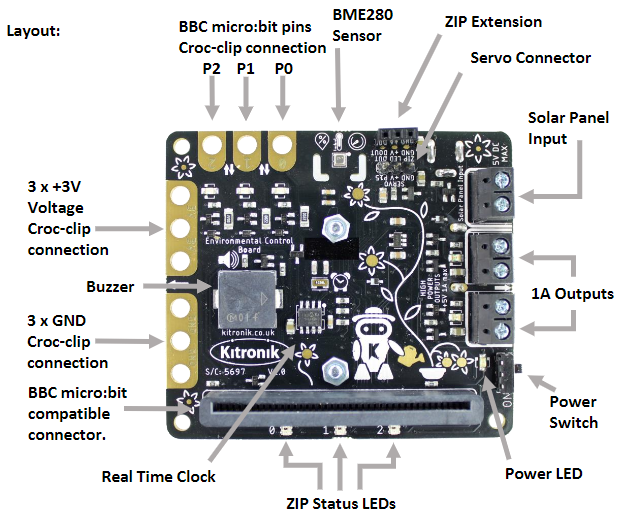
\includegraphics[scale=0.7]{Report/Images/KitronikBoardDiagram.png}
    \caption{Diagram of Kitronik Environmental Control board \cite{kitronikBoard}}
    \label{fig:KitronikDiagram}
\end{figure}

\begin{figure}[H]
    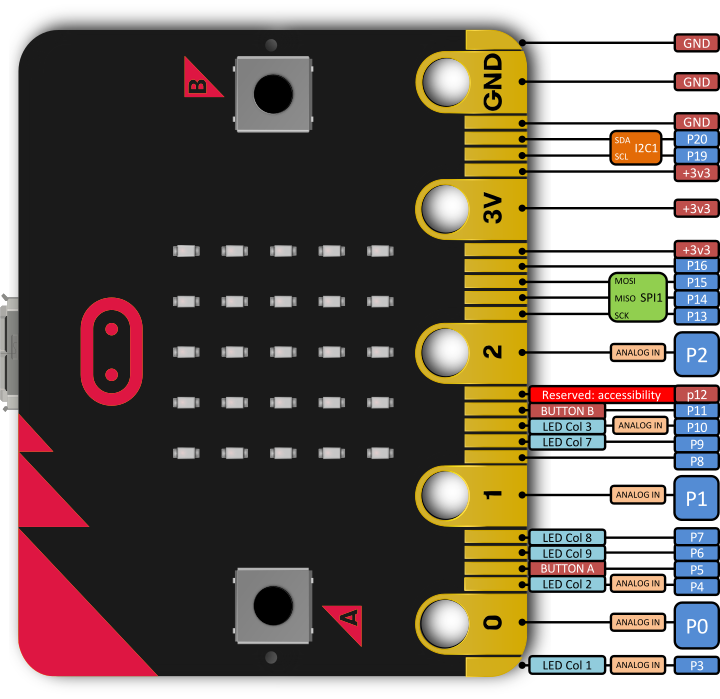
\includegraphics[scale=0.4]{Report/Images/MicrobitBoard.png}
    \caption{Diagram of Micro:bit board \cite{microbitDoc}}
    \label{fig:MicrobitBoard}
\end{figure}

\begin{figure}[H]
    \centering
    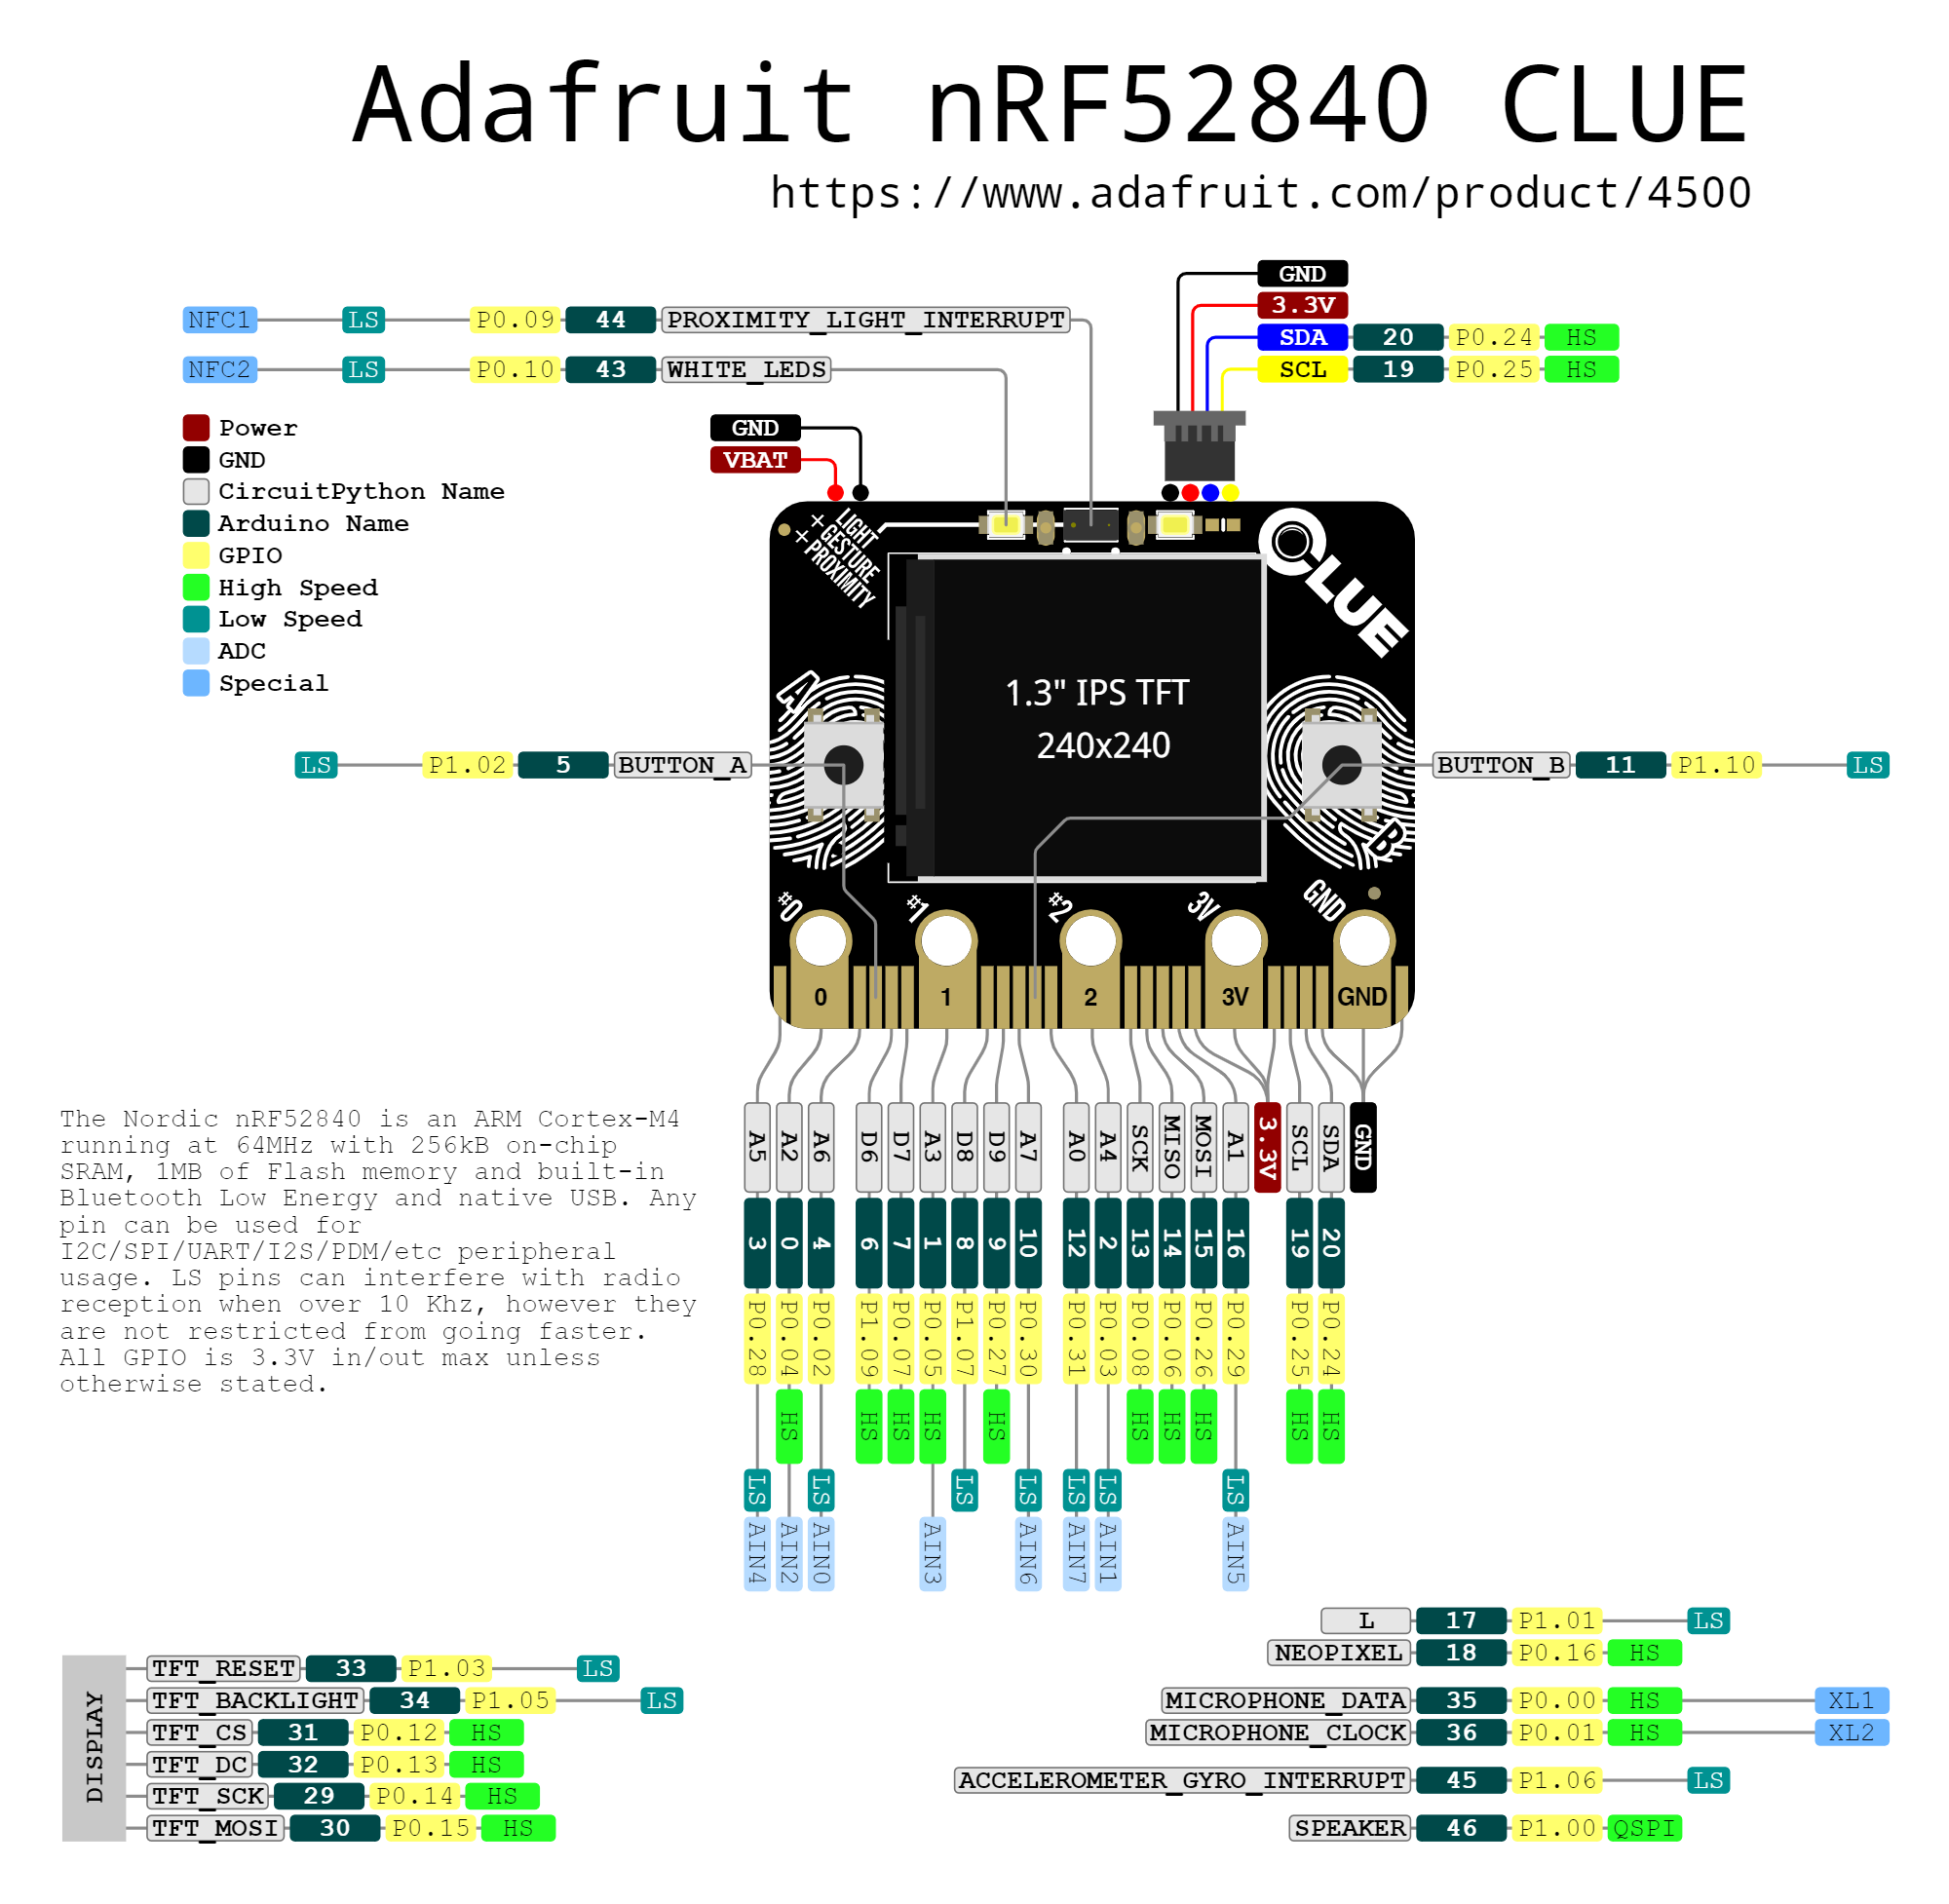
\includegraphics[scale=0.2]{Report/Images/ClueBoardDiagram.png}
    \caption{Diagram of Adafruit CLUE \cite{learnAdafruit}}
    \label{fig:CLUEDiagram}
\end{figure}

\begin{figure}[H]
    \centering
    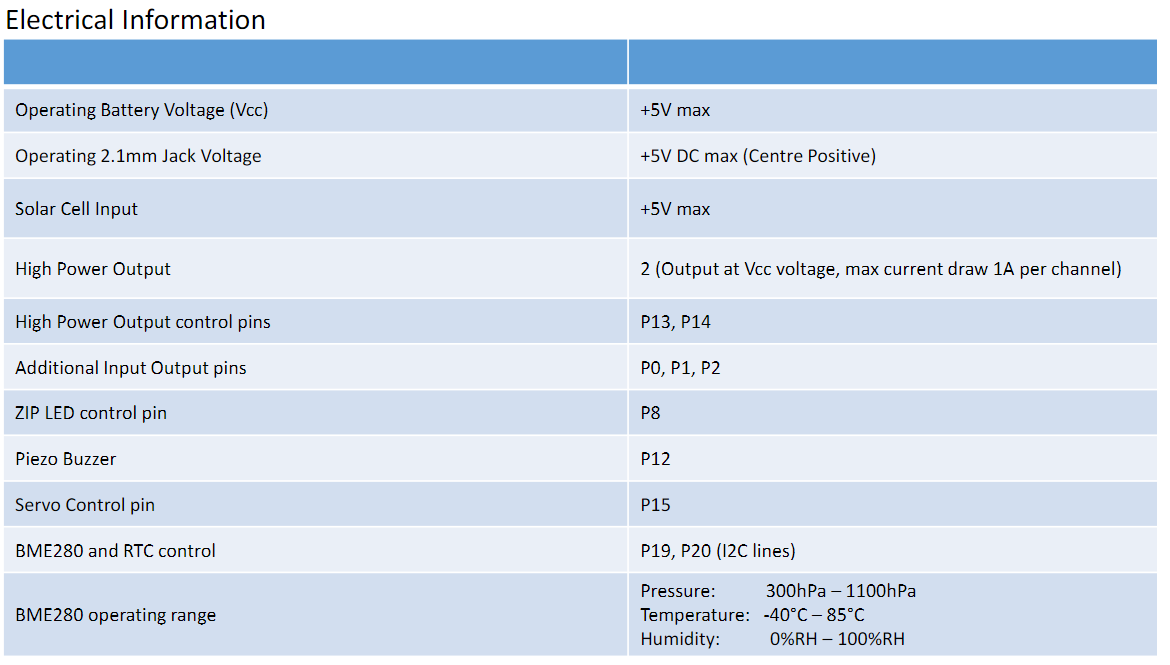
\includegraphics[scale=0.46]{Report/Images/KitronikInfoSheet.png}
    \caption{Environmental Control board datasheet \cite{kitronikBoard}}
    \label{fig:KitronikDatasheet}
\end{figure}

Using diagrams of the boards from their corresponding documentation plus the data sheet provided from the Kitronik kit, it was possible to see which pins on the Micro:bit match with the pins on the CLUE board without using trial and error:

\begin{center}
\begin{tabular}{| c | c | c | c | c | c | c | c |} 
    \hline
    \textbf{Micro:bit} & P0 & P1 & P2 & 3V & GND & P8 & P14\\
    \hline
    \textbf{CLUE} & A2 & A3 & A4 & 3.3V & GND & D8 & MISO\\
    \hline
\end{tabular}
\end{center}

On the Kitronik board, the pins P0, P1, P2 can all be used with crocodile clips to connect components such as the moisture sensor. The moisture sensor requires three crocodile clips: P0, 3V and GND. The ZIP LED has its own dedicated pins, which the datasheet specify uses P8. On the CLUE board this corresponds to the pin D8. Finally, the motor is a high voltage user and so is connected to pin P14 which corresponds to the pin MISO on the CLUE. The motor does not use crocodile clips, instead it is attached using two wires: positive and negative. These are stripped back slightly before being screwed into place (figure \ref{fig:KitronikDiagram}: the component labelled 1A outputs).

There are also a number of other built in sensors on both the Kitronik board and the CLUE:

\begin{itemize}
    \item Pressure sensor
    \vspace{-0.25cm}
    \item Thermometer
    \vspace{-0.25cm}
    \item Humidity sensor
    \vspace{-0.25cm}
    \item Light \& colour
    \vspace{-0.25cm}
    \item Sound etc.
\end{itemize}

\subsection{CircuitPython}

CircuitPython is a programming language made for using hardware. There are a number of libraries that make use of different components such as time, board and neopixel. For the experiments I will be using the following imports:

\begin{itemize}
    \item adafruit\_clue \cite{adafruitGit}
    \vspace{-0.25cm}
    \item rtc \cite{circPyDoc}
    \vspace{-0.25cm}
    \item time
    \vspace{-0.25cm}
    \item board
    \vspace{-0.25cm}
    \item neopixel \cite{neopixelGit}
    \vspace{-0.25cm}
    \item analogio
    \vspace{-0.25cm}
    \item digitalio
    \vspace{-0.25cm}
    \item microcontroller
\end{itemize}

The \textcolor{blue}{$adafruit\_clue$, $board$, $analogin$} and \textcolor{blue}{$digitalio$} imports allow me to specify which pins in the CLUE board to use when controlling the hardware.

e.g.
\begin{python}
    PIXEL_PIN = board.D8 
    analog_in = AnalogIn(board.A2)
    motor_pin = digitalio.DigitalInOut(board.MISO)
\end{python}

\textcolor{blue}{$rtc$} and \textcolor{blue}{$time$} are imported to control the time. In these experiments, time is used to hourly check if the plant needs watering, and to store the time and other parameters into a \textcolor{blue}{$.csv$} file. Lastly, \textcolor{blue}{$neopixel$} is the library used to control the ZIP LEDs on the top of the greenhouse.

To use all these libraries, I had to load them onto the CLUE board using a zip of up to date libraries on the CircuitPython website online \cite{circuitpython}. In the case of accidentally corrupting the board, this will need to be reloaded. And as the storage is only 2mb large, it is necessary to delete libraries that are not relevant to the project at hand. Especially as I will be storing data for the experiment on the board, there will need to be storage space as data will not be saved.

To load anything onto the board safely, you must be careful of not having any other power source connected to the CLUE board. It is also worth noting that nothing on the CLUE board should be updated directly. If a file (e.g. code) needs to be updated, then it is best to modify the code locally on your device, then replace the original file on the board.

\subsection{Storage}

Storing files generated by the code can be a little tricky for the Adafruit CLUE board. This is because it cannot allow multiple devices to simultaneously store files. Instead, the board has to specify only one device at a time can do so. 

First I had to create a \textcolor{blue}{$boot.py$} "which is executed before the USB connection is made" \cite{learnAdafruit}. The documentation for using the Adafruit CLUE supplied code to go into the file to set \textcolor{blue}{$readonly$} to \textcolor{blue}{$False$} on boot. The code in the boot file reads the input from pin D0. We can then use this as a switch for it we want to write via the code and or the USB. For my experiment, I set \textcolor{blue}{$readonly$} to \textcolor{blue}{$False$} when the pin is grounded, this way when the CLUE board is connected to the Kitronik board as part of the greenhouse, it will allow the code to write to file (which is necessary to log data).

\begin{python}[caption={boot.py}, captionpos=b]
    import board
    import digitalio
    import storage
    
    switch = digitalio.DigitalInOut(board.D0)
    switch.direction = digitalio.Direction.INPUT
    switch.pull = digitalio.Pull.UP

    storage.remount("/", switch.value)
\end{python}

Following the creation of \textcolor{blue}{$boot.py$}, learning how to write to file in code follows. This can be done by using \textcolor{blue}{$\textrm{open with}(x, y) \textrm{ as } z$} where \textcolor{blue}{$x$} is the file name, \textcolor{blue}{$y$} is the mode which determines whether what is being written to file appends the text or overwrites, and finally \textcolor{blue}{$z$} which is the variable name that will be used across the code when you are referring to the file. Nested in this block are methods \textcolor{blue}{$write$} and \textcolor{blue}{$flush$}  which are used on the file to log the data.

\begin{python}[caption={writing to file}, captionpos=b]
    try:
        with open("/experiment1.txt", "a") as fp:
            ... 
            fp.write("hello world")
            fp.flush()
            ...
    except OSError as e:
    ...
\end{python}

\subsection{Wiring the Board}

Setting up the greenhouse was a simple when using the instructional booklet that came with the set. First, the environmental board was wired up. This included using 3 sets of crocodile clips to connect the moisture sensor prongs. One wire was connected from the 0 pin on the moisture sensor to the 0 pin on the board. The second was connecting the 3v pins on the sensor to the board. Lastly, the GND pins on the sensor to the boards. The zip LEDs were connected to a tri-coloured set of wired that plugged straight into the designated area on the board. The motor for the water was a little more fiddly, requiring wire strippers to expose the inner wires in two thin cables. These were pushed into two small ports (negative and positive)) and then screwed into place.

Finally, the last set of crocodile clips were not used for any other components, but rather to allow the code to write to file. During the research phase, a \textcolor{blue}{$boot.py$} file was created to allow the code to write to file when a specified pin was grounded (the switch). So the final crocodile clip was connecting the 2 pin to GND so when the Adafruit CLUE board was inserted into the environmental board, the switch is on and the code is set to write mode.

One note to make about the equipment for the greenhouse is that the moisture sensor should not perform moisture check continuously, but rather occasionally as it can "promote rapid erosion of the electrodes".

% Add picture of the board's setup

\subsection{Creating the Environment}

% Mention how I created each environment
% The soil and whatnot that create the greenhouse
% Maybe mention the batteries? Make sure it's not too repetitive

\subsection{The Test Round}

The development of the code for the experiments consisted of using a number of constants throughout. This way, when developing the code for the next set of experiments, there only needed to be minor adjustments to the values of the constants. To ensure the code was working, I ran a test experiment. This was for a number of reasons such as making sure all the components were working, there wasn't too much of a delay for the time and the cress will grow a significant amount during that time.

Experiment number one (test) was with white light and a constant moisture level of 0.5v. Many unexpected events occurred during this week long time period. The greenhouse was kept in a small box to prevent other light sources affecting the course of the experiment, this was also to protect the greenhouse from physical damage such as item falling onto it and damaging the components. Within the first 24 hours of the project, a check was performed to find that the white light had turned red. The first assumption made was that the blue and green LED lights had broken, but it was decided that the project should keep running to find any other defects. A few hours later, the greenhouse was checked again to see that the screen of the Adafruit CLUE had turned off. Again another assumption was made that the screen was on standby, perhaps because nothing on the screen was changing. At the time, the code of the experiment did not print anything to screen, which was noted and to be changed for the next set of experiments. It was later found that the CLUE board did not record any information past the 6 hours that it remained awake (the \textcolor{blue}{$.csv$} file only contained 6 rows of information). On the sixth day of the experiment, the red light had fully died as well. This was the sign that the first experiment had ended. 

% Add pictures of the first experiment (20221230)

After concluding the first round had finished, it was time to measure all the different parts of the cress:

\begin{itemize}
    \item Leaf span
    \vspace{-0.25cm}
    \item Stem height
    \vspace{-0.25cm}
    \item Root length
\end{itemize}

All these measurements were taken taken by hand with a clear Oxford ruler and a clean wooden desk, and results stored in a spreadsheet for later use. For the first experiment, a spreadsheet was made to see the kind of data was being stored.

\begin{figure}[H]
    \centering
    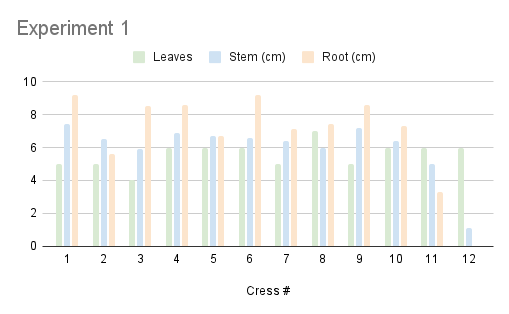
\includegraphics[scale=0.8]{Report/Images/Experiment1.png}
    \caption{Graph of results for experiment 1}
    \label{fig:experiment1}
\end{figure}

Although all the experiments' results will be concluded in the evaluation, it was important to check the results of the first test experiment immediately. In figure \ref{fig:experiment1}, we can conclude that the value for leaves did not vary by much cress to cress. Especially as the cress with fewer leaves often looked as if their leaves had yet to unfurl. In the spreadsheet, number of leaves was then changed to leaf span. For the last cress (cress number 12 in the diagram), the measurement of the stem and root were abnormally short. This anomaly was likely caused by the moisture sensory hindering its growth by being in the way. This then meant another change was to made to the experiments: the moisture sensor should be on the side of the tray of soil and out of the way of any of the seeds to prevent obstruction of growth.

Back to the running of the test experiment, it was also easy to conclude that the motor had been working fine as there were droplets of water found on the cress, and the soil was far from dry. However, it did seem that the soil was more wet than necessary as the \textcolor{blue}{$.csv$} file was returning high values for the moisture levels of the soil. This lead to another change in the code to pulse the motor on and off, giving the water time to spread through the soil and reach the moisture sensor before flooding the tray.

All that was left was the find the issue causing the LEDs to not work and the CLUE board to stop recording measurements. After testing all the hardware individually, it was discovered that the batteries needed replacing. This was a massive drawback in the board as there were at least 6 rounds of experiments to go and replacing the batteries every week is costly and bad for the environment. After a little more research into the board \cite{kitronikBoard}, there seemed to be a DC connected that could power the board straight from a socket. This allowed the board to be powered for the entirety of the project length without the need to purchasing and disposing of new AA batteries every week, as well as being a more reliable source of power. it is important to note that electricity often comes from fossil fuels which is not particularly eco-friendly either, but is better than disposing of lithium batteries at such a frequent rate.

\subsection{The Experiments}

The rest of the experiments performed without any other technical issues. The second experiment (the control experiment) was of white light and a moisture level of 0.5v. One seed did get lost in the soil (had not grown) and another barely germinated, having only a small stem visibly coming out of the seed with no root or leaves. The cress itself looked entirely different, with stronger stems and being able to hold themselves up. The green colour on the leaves and the stems was also a lot more vibrant compared to the first test experiment where the stems were white and the leaves a little paler.

% add picture of experiment 2 (20230106)
% Add the picture of all of them growing, the picture of it on the table and the picture of the seed

Experiment number three consisted of a constant blue light with a moisture level of 0.5v. The roots for this round were a lot larger than any of the other two, the longest reaching almost a foot long. They were extremely fine and hard to capture on camera. The leaves at the top were also a different shape, having a longer split in the stem before the leaves appeared. This made the averages of the leaf span a lot larger.

% Add picture (20230114)
% The leaf span and the ft long root

Experiment four used red light with the same 0.5v moisture. The roots were shorter and less fragile looking, with little fuzzy edges (unfortunately, the texture was too fine to pick up on camera). The leaves grew a little closer together and where more narrow compared to the long split in the blue light experiment.

% Add any pictures?

The no light experiment surprisingly grew taller than expected, yet the leaves had barely sprouted and the colour was more yellow than green. The stems grew very straight, likely as there was no light source to grow towards and the roots and stems were very similar lengths (compared to other experiments where there was often a big difference).

% pictures somewhere of the leaves being pale af

Experiment number six was for a lower moisture level in the soil set to 0.2v. This ended up different to the original plan of the last two experiment both being an increase in moisture. The reason being that 0.5v was alright leading to fairly moist soil for all the different light experiments. Instead, the final two experiments will consist of one lower moisture level and one higher. In this sixth round, the leaves where a little paler than the other rounds and a lot more delicate. The leaves did not spread very far and the roots grew a lot more than the other experiments. They did not have a longer average length than that of experiment 3, but rather, the roots where more than just one single strand like the other rounds. They took over the soil and were had to break apart for when it was time to measure them. Because of this, the root measurements may not be accurate as they may have ripped at the extraction stage. Another interesting thing to note is that the stems were more soft and unable to hold the weight of the cress as well.

% should be some images of the dry soil and the roots taking over

Lastly experiment number seven is with a white light and and moisture level set to 2.5v. The soil for the round was very wet, but considering cress can be grown using hydroponics, this should not be an issue. There are plenty of plants where soaking the seeds too long can cause them to drown. After six days, the cress had grown well, and wasn't much different than the control round which had less water. This shows that cress is fairly tolerant to high levels of water in their surrounding soil.


\section{Kitronik Library Development}

The idea behind creating a library for the Kitronik greenhouse kit is to make it easier for people using an Adafruit CLUE to create experiments and enjoy using the greenhouse. This single library will make code a lot easier and cleaner as there is less setting up and fewer imports to make. To implement this code, I will be creating a facade as an interface to all the imports needed. The interface itself will make use of the imports to set up the pins for all the hardware. This will require users to ensure they use the right pins for each component. To test this library does reduce complexity, I will be recreating the experiment code for the control round using the new library and comparing the code to the original version. Finally, I will be converting the file to \textcolor{blue}{$.mpy$} as all libraries on the CLUE board are of this format. \textcolor{blue}{$.mpy$} files contain bytecode of precompiled program from a Python source file \cite{micropython}. This can be done by using a program called \textcolor{blue}{$mpy-cross$}.

\subsection{Creating the Interface}

Creating the interface for the library initially including importing all the modules necessary for controlling the components that come with the greenhouse kits. This was then followed by the setting up of all the components. This includes specifying the pins for each piece of hardware, the number of lights on the zip LED and other small details needed to run code using these tools.

What came next was creating all the public functions that users can interact with. These were just basic controls for each hardware such as turning on and off the motor and getting values for the temperature and moisture level. For code that is designed for public use, documentation is a vital element of the interface. Each function required its own comment specifying its purpose, the parameters it takes and any return types. This needs to be concise yet understandable to beginners.

The more complex part of the code was simplifying the use of the LEDs. The ideal functionality is to allow the users to either control all of the lights simultaneously, or individually. This can be setting different colours to each pixel of light, or turning on only a few of them, but not all of them. More functionality that was added was timers for certain components. When creating the code for the experiments, the motor for the water was only used in short bursts, and not for one long period of time. Instead of the user importing the \textcolor{blue}{$time$} module, the user can call \textcolor{blue}{$motorTimer$} and specify a time in seconds for the motor to be turned on for. This was also added for the LED lights. Although simple, this functionality was added to the experiment's code after realising that the motor pumping water for a long period of time made the measurements for the moisture sensor less accurate as the water needed time to absorb into the soil and around the area the sensor was sitting. As for the LEDs, the timer can be used to create a cycle of night and day for the growing environment. 

\subsection{CookieCutter}

CookieCutter is a "command-line utility that creates projects from cookiecutters" \cite{cookiecutter}. It creates a template for Python libraries and can be used on Python version 3.7 and newer. To use, it must first be installed using the terminal (Linux in this case). Following this, the command to run CookieCutter is used. This returns a list of prompts that must be entered about the project. The text that is entered is used in the template comments regarding authors of the project, sponsored companies and more.

\begin{python}[caption={Installing CookieCutter on Linux}, captionpos=b]
    pip install cookiecutter
    cookiecutter gh:adafruit/cookiecutter-adafruit-circuitpython
\end{python}

Once CookieCutter has created the template file, all that is left is to copy and paste the library code that has been created into the\textcolor{blue}{$.py$} file that has been created. The purpose of this is to provide documentation on Github for other users. It includes a licenses folder for all the necessary Copyright files and example code files to understand how the library works.

\subsection{mpy-cross}

To use the library, it is preferred to have the \textcolor{blue}{$.py$} source code converted to a \textcolor{blue}{$.mpy$}. This is just as easy to import but is the precompiled version of the code. To create this package, \textcolor{blue}{$mpy-cross$} must first be downloaded \cite{libraryFileTypes} \cite{mpycrossDownloads}. The download is renamed to \textcolor{blue}{$mpy-cross$} and moved to the directory containing the Python source code. Ensuring the terminal is in the same directory as the \textcolor{blue}{$mpy-cross$} file and the source code, the following line must be entered into the terminal (where the path to the source code is changed accordingly).

\begin{python}
    ./mpy-cross path/to/your-library-file.py
\end{python}

To use the \textcolor{blue}{$.mpy$} file, it's as easy as copying it to your CIRCUITPY drive and importing the correct file name in the code. As it is bytecode, whitespace and comments are not included, which makes the file a lot smaller than using the Python source code file. As with any bytecode program, it does not need to be compiled again, and therefore uses less RAM on the board when compiling the entire program \cite{libraryFileTypes}.
